\documentclass[8pt]{beamer}

\usepackage{import}
\usepackage{graphicx}
\usepackage{tcolorbox}
\usepackage{listings}

%\begin{tcolorbox}
%Contenu de la boite.
%\end{tcolorbox}
%\begin{tcolorbox}[title=Titre de la boite]
%Contenu de la boite.
%\end{tcolorbox}

%\begin{tcolorbox}[
%rightrule=3mm,
%colback=red!5!white,
%colframe=red!75!black,
%arc=0mm,
%aftertitle={\hfill\colorbox{blue!50!black}{approved}},
%title={\bfseries Titre de la boite}
%]
%This is a \textbf{tcolorbox}.
%\end{tcolorbox}

\makeatletter
\long\def\beamer@section[#1]#2{%
  \beamer@savemode%
  \mode<all>%
  \ifbeamer@inlecture
    \refstepcounter{section}%
    \beamer@ifempty{#2}%
    {\long\def\secname{#1}\long\def\lastsection{#1}}%
    {\global\advance\beamer@tocsectionnumber by 1\relax%
      \long\def\secname{#2}%
      \long\def\lastsection{#1}%
      \addtocontents{toc}{\protect\beamer@sectionintoc{\the\c@section}{#2\hfill\the\c@page}{\the\c@page}{\the\c@part}%
        {\the\beamer@tocsectionnumber}}}%
    {\let\\=\relax\xdef\sectionlink{{Navigation\the\c@page}{\noexpand\secname}}}%
    \beamer@tempcount=\c@page\advance\beamer@tempcount by -1%
    \beamer@ifempty{#1}{}{%
      \addtocontents{nav}{\protect\headcommand{\protect\sectionentry{\the\c@section}{#1}{\the\c@page}{\secname}{\the\c@part}}}%
      \addtocontents{nav}{\protect\headcommand{\protect\beamer@sectionpages{\the\beamer@sectionstartpage}{\the\beamer@tempcount}}}%
      \addtocontents{nav}{\protect\headcommand{\protect\beamer@subsectionpages{\the\beamer@subsectionstartpage}{\the\beamer@tempcount}}}%
    }%
    \beamer@sectionstartpage=\c@page%
    \beamer@subsectionstartpage=\c@page%
    \def\insertsection{\expandafter\hyperlink\sectionlink}%
    \def\insertsubsection{}%
    \def\insertsubsubsection{}%
    \def\insertsectionhead{\hyperlink{Navigation\the\c@page}{#1}}%
    \def\insertsubsectionhead{}%
    \def\insertsubsubsectionhead{}%
    \def\lastsubsection{}%
    \Hy@writebookmark{\the\c@section}{\secname}{Outline\the\c@part.\the\c@section}{2}{toc}%
    \hyper@anchorstart{Outline\the\c@part.\the\c@section}\hyper@anchorend%
    \beamer@ifempty{#2}{\beamer@atbeginsections}{\beamer@atbeginsection}%
  \fi%
  \beamer@resumemode}%

\def\beamer@subsection[#1]#2{%
  \beamer@savemode%
  \mode<all>%
  \ifbeamer@inlecture%
    \refstepcounter{subsection}%
    \beamer@ifempty{#2}{\long\def\subsecname{#1}\long\def\lastsubsection{#1}}
    {%
      \long\def\subsecname{#2}%
      \long\def\lastsubsection{#1}%
      \addtocontents{toc}{\protect\beamer@subsectionintoc{\the\c@section}{\the\c@subsection}{#2\hfill\the\c@page}{\the\c@page}{\the\c@part}{\the\beamer@tocsectionnumber}}%
    }%
    \beamer@tempcount=\c@page\advance\beamer@tempcount by -1%
    \addtocontents{nav}{%
      \protect\headcommand{\protect\beamer@subsectionentry{\the\c@part}{\the\c@section}{\the\c@subsection}{\the\c@page}{\lastsubsection}}%
      \protect\headcommand{\protect\beamer@subsectionpages{\the\beamer@subsectionstartpage}{\the\beamer@tempcount}}%
    }%
    \beamer@subsectionstartpage=\c@page%
    \edef\subsectionlink{{Navigation\the\c@page}{\noexpand\subsecname}}%
    \def\insertsubsection{\expandafter\hyperlink\subsectionlink}%
    \def\insertsubsubsection{}%
    \def\insertsubsectionhead{\hyperlink{Navigation\the\c@page}{#1}}%
    \def\insertsubsubsectionhead{}%
    \Hy@writebookmark{\the\c@subsection}{#2}{Outline\the\c@part.\the\c@section.\the\c@subsection.\the\c@page}{3}{toc}%
    \hyper@anchorstart{Outline\the\c@part.\the\c@section.\the\c@subsection.\the\c@page}\hyper@anchorend%
    \beamer@ifempty{#2}{\beamer@atbeginsubsections}{\beamer@atbeginsubsection}%
  \fi%
  \beamer@resumemode}

%\addtobeamertemplate{navigation symbols}{}{%
    \usebeamerfont{footline}%
    \usebeamercolor[fg]{footline}%
    \hspace{1em}%
    \insertframenumber/\inserttotalframenumber
}
\setbeamercolor{footline}{fg=blue}
\setbeamerfont{footline}{series=\bfseries}

\expandafter\def\expandafter\insertshorttitle\expandafter{%
  \insertshorttitle\hfill%
  \insertframenumber\,/\,\inserttotalframenumber}




%\usetheme{Copenhagen}
\usetheme{Antibes}

\AtBeginSubsection[]
{
\begin{frame}<beamer>{Table of Contents}
  %\begin{tiny}
  \tableofcontents[
    currentsubsection,
    subsubsectionstyle={show/show/shaded/shaded}
  ]
  %\end{tiny}
\end{frame}
}

% https://www.overleaf.com/learn/latex/Code_listing
\lstdefinestyle{mycodestyle}{
%  backgroundcolor=\color{backcolour},
%  commentstyle=\color{codegreen},
%  keywordstyle=\color{magenta},
%  numberstyle=\tiny\color{codegray},
%  stringstyle=\color{codepurple},
  basicstyle=\ttfamily\footnotesize,
  breakatwhitespace=true,
  breaklines=true,
  captionpos=b,
  keepspaces=false;
  numbers=left,
  numbersep=0pt,
  showspaces=false,
  showstringspaces=false,
  showtabs=false,
  tabsize=2
}
\lstset{style=mycodestyle}

\title{K8S - sum-up}
\subtitle{Beamer's powa}
\author{Florian}
\institute{Tourism's institute of nowhere}
\date{\today}

\makeatother
\begin{document}

\begin{frame}
\titlepage{}
\end{frame}

\begin{frame}<beamer>{Table of Contents}
  \tableofcontents[]
\end{frame}

\section{Core concept}

\subsubsection{k8s architecture}
\begin{frame}{k8s architecture}
\begin{columns}
\begin{column}{0.2\textwidth}
\end{column}
\begin{column}{0.8\textwidth}
  \begin{itemize}
  \item \textbf{Master} Control plane (+ ETCD)
    \begin{itemize}
    \item[kube-apiserver]: Auth and etcd's communication (static)
    \item[kube-controller-manager]: Keep the system in desired state (static)
    \item[kube-scheduler]: Deals pods on nodes (static)
    \item[kubelet]: Manage controller order (package)
    \item[kube-proxy]: Manage services (daemonset)
    \end{itemize}
  \item \textbf{Worker} Workload
    \begin{itemize}
    \item[kubelet]: Manage controller order (package)
    \item[kube-proxy]: Manage services (daemonset)
    \end{itemize}
  \item \textbf{(ETCD)} (static)
  \end{itemize}
  \begin{itemize}
    \item Static pod:
    \begin{itemize}
      \item Deployed on node file system \texttt{/etc/kubernets/manifest}
      \item can be reconized by \texttt{<pod\_name>-<node\_name>}
    \end{itemize}
\end{itemize}
\end{column}
\end{columns}
\end{frame}

\subsubsection{Deployment workflow (my vision)}
\begin{frame}{Deployment workflow (my vision)}
  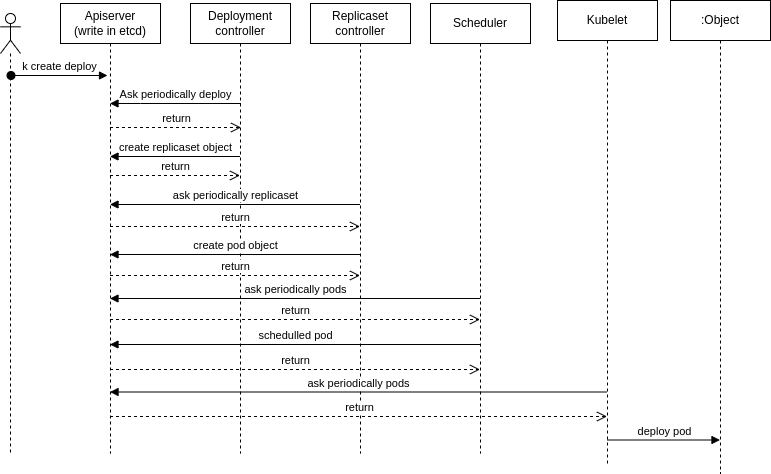
\includegraphics[width=1\linewidth]{assets/k8s-deploy-creation-drawio.png}
\end{frame}


\section{Pods and co}
\subsection{How to deploy}

\subsubsection{Pods command}
\begin{frame}[fragile]{\subsubsecname}
\begin{itemize}
  \item \textbf{(po) minimal}: \texttt{k run <pod\_name> --image=<image\_name>}
  \item \textbf{(po) example}: \texttt{k run toto-frontend --image=nginx -l "app=toto,tier=frontend" --dry-run=client -o yaml}
  \item \textbf{(po) connection}: \texttt{k exec -it <pod\_name> -- <command>}
  \item \textbf{(po) interaction}: \texttt{k [get|describe|edit|delete] [pods|po] <pods\_name>}
  \begin{itemize}
    \item in \texttt{get} command ready: container in pod ready/container total in pod
  \end{itemize}
  \item \textbf{(po) edition} can only edit 4 field (if edit anything else: delete/recreate)
  \begin{itemize}
    \item spec.containers[*].image
    \item spec.initContainers[*].image
    \item spec.activeDeadlineSeconds
    \item spec.tolerations
  \end{itemize}
  \item \textbf{(po) get yaml} \texttt{k get pods <pods\_name> -o yaml > <pods\_name>.po.yaml}
  \item \textbf{(po) create from yaml} \texttt{k apply -f <pods\_name>.po.yaml}
  \item \textbf{(po) delete from yaml} \texttt{k delete -f <pods\_name>.po.yaml}
\end{itemize}

\end{frame}

\subsubsection{Replicasets and Deployments}
\begin{frame}{Replicasets and Deployments}

  \begin{itemize}
    \item \textbf{(rs) interaction}: \texttt{k [get|describe|edit|delete] [replicasets|rs] <rs\_name>}
    \item \textbf{(ds) interaction}: \texttt{k [get|describe|edit|delete] [daemonsets|ds] <ds\_name>}
    \item \textbf{(deploy) minimal}: \texttt{k create deploy <deploy\_name> --image=<image\_name>}
    \item \textbf{(deploy) interaction}: \texttt{k [get|describe|edit|delete] [deployments|deploy] <deploy\_name>}
    \item \textbf{(rs|deploy) scaling}: \texttt{k scale [rs|deploy] <rs|deploy\_name> --replicas=<number>}
    \item free edition for rs and deploy
    \begin{itemize}
      \item after rs edition need to delete pod to create new version
      \item deploy have update policy
    \end{itemize}
    \item replicasets: be sure to have the good number of a pod
    \item daemonsets: be sure to have the pod on all node
    \item deployment: be sure to have the pod as defined
  \end{itemize}
  
\end{frame}

\subsubsection{Yaml comparaison}
\begin{frame}[fragile]{Yaml comparaison}

\begin{small}
\begin{columns}
  \begin{column}{0.20\linewidth}
    \textbf{toto.po.yaml}
    \begin{lstlisting}








apiVersion: v1
kind: Pod
metadata:
  labels:
    run: toto
  name: toto
spec:
  containers:
  - image: nginx
    name: toto
    \end{lstlisting}
  \end{column}
  \begin{column}{0.27\linewidth}
    \textbf{toto.rs.yaml}
    \begin{lstlisting}
apiVersion: apps/v1
kind: ReplicaSet
metadata:
  labels:
    app: toto
  name: toto
spec:
  selector:
    matchLabels:
      app: toto
  template:
    metadata:
      labels:
        app: toto
    spec:
      containers:
      - image: nginx
        name: nginx
  replicas: 1
  \end{lstlisting}
  \end{column}
  \begin{column}{0.26\linewidth}
    \textbf{toto.ds.yaml}
    \begin{lstlisting}
apiVersion: apps/v1
kind: DaemonSet
metadata:
  labels:
    k8s-app: ingress
  name: kube-proxy
spec:
  selector:
    matchLabels:
      k8s-app: ingress
  template:
    metadata:
      labels:
        k8s-app: ingress
    spec:
      containers:
      - image: nginx
        name: nginx
    \end{lstlisting}
  \end{column}
  \begin{column}{0.27\linewidth}
    \textbf{toto.deploy.yaml}
    \begin{lstlisting}
    apiVersion: apps/v1
    kind: Deployment
    metadata:
      labels:
        app: toto
      name: toto
    spec:
      selector:
        matchLabels:
          app: toto
      template:
        metadata:
          labels:
            app: toto
        spec:
          containers:
          - image: nginx
            name: nginx
      replicas: 1
    \end{lstlisting}
  \end{column}
\end{columns}
\end{small}
\end{frame}

\subsubsection{Multicontainer Pod}
\begin{frame}[fragile]{\subsubsecname}
  \begin{itemize}
  \item sidecar (log, metric scraper)
  \item adapter
  \item ambassador
  \end{itemize}
\end{frame}

\subsubsection{Kubectl proxy and port forward}
\begin{frame}[fragile]{Kubectl proxy and port forward}
  \begin{itemize}
  \item If you try to access apiserver, you need authent
  \item \texttt{kubectl proxy}: permit to acces apiserver and expose in on localhost:8001
  \item \texttt{curl http://localhost:8001/api/v1/namespaces/default/services/nginx/proxy/}
  \item unless exposition you cannot access pod from outside the cluster
  \item \texttt{kubectl port-forward service/nginx 28080:80}
  \item can be use pod, deploy, svc
  \end{itemize}
\end{frame}


\subsection{How to list}

\subsubsection{Kubectl version tricks}
\begin{frame}[fragile]{\subsubsecname}
  \begin{itemize}
    \item \texttt{k versions}: cluster version
    \item \texttt{k api-versions}: all version supported by the cluster
    \item \texttt{k api-resources}: list ressource, shortcut, apigroup
    \item \texttt{k explain <resource>}: describe a resource and give recommended version
    \item \texttt{k explain <resource> --recursive}: give all key off a resource
  \end{itemize}
\end{frame}

\subsubsection{Kubectl output format}
\begin{frame}[fragile]{\subsubsecname}
  \begin{itemize}
    \item \texttt{k get <resource>}: list the resource
    \item \texttt{k get <resource> <specific resource>}: retourn only the specific resource targeted
    \item \texttt{k get <resource> -o wide}: generally give more detail
    \item \texttt{k get <resource> -o json}: return data in json format
    \item \texttt{k get po nginx -o yaml}: return data in yaml format
    \item \texttt{k get <resource> --show-labels}: show labels in the list
  \end{itemize}
  Good but not detailed here
  \begin{itemize}
    \item \texttt{k get <resource> -o jsonpath='{.items[*].metadata.name}'}
    \item \texttt{k get no -o jsonpath='{.items[?(@.metadata.name == "node01")].status.nodeInfo.osImage}'}
    \item \texttt{k get no -o custom-columns='NAME:.metadata.name, OS:.status.nodeInfo.osImage'}: print column of your choice
    \item \texttt{k get po -l "tier=front,app=ldap"}: filter by label
  \end{itemize}
\end{frame}


\subsection{Command and args}

\subsubsection{Command and args}
\begin{frame}[fragile]{\subsubsecname}
  \begin{itemize}
    \item \texttt{command} in yaml file will surcharge \texttt{entrypoint} in dockerfile
    \item \texttt{args} in yaml file will surcharge \texttt{command} in dockerfile
  \end{itemize}
  \begin{lstlisting}
    ---
    apiVersion: v1
    kind: Pod
    metadata:
      labels:
        run: toto
      name: toto
    spec:
      containers:
      - image: ubuntu
        name: toto
        command:
        - sleep
        args:
        - "1200"
\end{lstlisting}
\end{frame}


\subsection{Storage}

\subsubsection{Storage architecture}
\begin{frame}[fragile]{\subsubsecname}
  \begin{itemize}
    \item \texttt{volumeMount} connect a pod to a \texttt{volume}
    \item \texttt{volume} is linked to a \texttt{Persistent Volume Claim} (not only)
    \item \texttt{PVC} claim the reservation of a \texttt{Persistent Volume}
    \item \texttt{PVC} constraint are
    \begin{itemize}
      \item sufficient Capacity
      \item Access Modes
      \item Volumes Modes
      \item (Storage Class)
      \item (Selector)
    \end{itemize}
    \item \texttt{PV} give a place to store
    \item \texttt{Storage Class} generate dynamically \texttt{Persistent Volume}
  \end{itemize}
\end{frame}

\subsubsection{Storage implementation}
\begin{frame}[fragile]{Storage implementation}
\begin{small}
\begin{columns}
  \begin{column}{0.33\linewidth}
    \begin{lstlisting}
---
apiVersion: v1
kind: Pod
metadata:
  labels:
    run: toto
  name: toto
spec:
  containers:
  - image: ubuntu
    name: toto
    volumeMounts: # <----
    - mountPath: /opt
      name: data-volume
  volumes: # <----
  - name: data-volume
    persistentVolumeClaim: # <----
      claimName: myclaim
    \end{lstlisting}
  \end{column}

  \begin{column}{0.33\linewidth}
    \begin{lstlisting}
---
apiVersion: v1
kind: PersistentVolumeClaim # <----
metadata:
  name: myclaim
spec:
  accessModes:
    - ReadWriteOnce
  resources:
    requests:
      storage: 500Mi
    \end{lstlisting}
  \end{column}

  \begin{column}{0.33\linewidth}
    \begin{lstlisting}
---
apiVersion: v1
kind: PersistentVolume # <----
metadata:
  name: pv-vol1
spec:
  # ReadOnlyMany, ReadWriteOnce, ReadWriteMany
  accessModes:
    - ReadWriteMany
  capacity:
    storage: 12Gi
  # or replace with storage provider
  hostPath:
    path: /tmp/data
  # Retain or Recycle or Delete
  persistentVolumeReclaimPolicy: Retain
      \end{lstlisting}
  \end{column}
\end{columns}
\end{small}
\end{frame}


\begin{frame}[fragile]{Todo}
\begin{itemize}
\item[todo] Kubectl proxy and port forward (ckad)(cks)
\item[app access] service (Nodeport, clusterIp) (ckad)(cka)
* DNS (cka)
* Ingress (ckad)(cka)(cks)
\item[config] Config map (ckad)(cka)
* Env vars (ckad)(cka)
* Secrets (generic, docker-registry) (ckad)(cka)
\item[scheduling] namespace (ckad)(cka)
* Rolling update and rollback (ckad)(cka)
* Taint and toleration (ckad)(cka)
* Node affinity (ckad)(cka)
* Node selector (ckad)(cka)
\item[vrac] Logs (ckad)(cka)
* Blue Green deployment (ckad)
* Canary Deployment (ckad)
* Jobs (ckad)
* CronJob (ckad)
* initcontainer (cka)
* Security context (ckad)(cka)(cks)
* etcd (cka)
* Scheduling (cka)
* Metrics (ckad)
* Cluster port (cka)
* Request and limits (in pods and limitrange) (ckad)(cka)
* Cluster update (cka)(cks)
* Cluster install (cka)
* Cluster Backup and restore (cka)
* Security primitive (cka)(ckS)
* k8s certificate (cka)(cks)
* Certificate Signing Request CSR (cka)(cka)
* API Group (ckad)(cka)(cks)
* Authorization (ckad)(cka)(cks)
* Role Base RBAC (ckad)(cka)(cks)
* Cluster Role (ckad)(cka)(cks)
* Service Account (ckad)(cka)(cka)
* Default Admission Controller (ckad)(cks)
* Validating and Mutating Admission Controllers (ckad)(cks)
* Network Policy NetPol (ckad)(cka)(cks)
* Kubeconfig (ckad)(cka)(cks)
* API Version (ckad)
* CNI (cka)
* ReadinessProbe and LivenessProbe (ckad)
* Docker Image (ckad)
* Operator Framework (CRD + Custom Controller) (ckad)
* Helm (ckad)
* Authentication (cka)(cks)
\item[security] CIS Linux (cks)
* CIS k8s (cks)
* Kube bench (cks)
* TLS (cka)(cks)
* Kubelet security (cks)
* Dashboard (cks)
* Securing Dashboard (cks)
* Docker service conf and securing (cks)
* Limite node access (cks)
* SSH Hardening (cks)
* Kernel Module Restriction (cks)
* Disable Port (cks)
* Firewall Basics (cks)
* Syscalls and seccomp (cks)
* Syscalls - AquaSec Tracee (cks)
* AppArmor (cks)
* Pod Security Policy PSP (cks)
* Open Policy Agent (cks)
* Secret Management (cks)
* gVisor (cks)
* kataContainer (cks)
* Runtime class (cks)
* One way SSL, mutual SSL (cks)
* image policy webhook (cks)
* Kubesec (cks)
* Trivy (cks)
* Falco (cks)
* Immutability (cks)
* Audit log (cks)
\end{itemize}
\end{frame}


\end{document}
